\documentclass[dvipdfmx,a4paper,11pt]{jsarticle}

\usepackage[dvipdfmx]{graphicx}
\usepackage{amsmath}
\usepackage{listings}
\usepackage{xcolor}
\usepackage{here}

\lstset{
  basicstyle=\ttfamily\small,
  frame=single,
  numbers=left,
  breaklines=true,
  keywordstyle=\color{blue},
  commentstyle=\color{green!50!black},
  stringstyle=\color{red}
}

\title{ナップサック問題における総当たり法と動的計画法の比較}
\author{氏名：玉城　俐空}
\date{\today}

\begin{document}

\maketitle
\newpage
\tableofcontents
\newpage

\section{内容}

本レポートでは、ナップサック問題を対象として、総当たり法と動的計画法（DP）による解法を実装し、それぞれの考え方と計算量について考察する。

ナップサック問題とは、複数の品物について、それぞれ重さと価値が与えられているとき、重さの上限を超えない範囲で価値の合計が最大となるような品物の組み合わせを求める問題である。

\section{問題設定}

本課題では、以下の重さと価値をもつ品物について、重さの合計が45以下となる範囲で価値の合計が最大となる組み合わせを求める。

\begin{lstlisting}[language=Python, caption=問題で用いるデータ]
Weight = [4,8,3,5,9,2,3,1,5,2,4,2,7,10,3,13,11,8,5,2,4,5,6]
money  = [6,12,4,3,7,1,3,2,7,3,4,2,10,13,5,16,14,9,1,4,6,2,4]

W = 45
\end{lstlisting}

ここで、\texttt{Weight} は各品物の重さ、\texttt{money} は各品物の価値、\texttt{W} はナップサックに入れられる重さの上限を表す。

\section{総当たり法}

総当たり法では、各品物について「選ぶ」または「選ばない」の2通りをすべて試す。品物の数を $n$ とすると、全ての組み合わせの数は

\[
2^n
\]

である。

今回の問題では品物数が23個であるため、調べる組み合わせ数は

\[
2^{23}
\]

通りとなる。

\begin{lstlisting}[language=Python, caption=総当たり法による実装]
import time

start = time.perf_counter()

Weight = [4,8,3,5,9,2,3,1,5,2,4,2,7,10,3,13,11,8,5,2,4,5,6]
money  = [6,12,4,3,7,1,3,2,7,3,4,2,10,13,5,16,14,9,1,4,6,2,4]

W = 45
n = len(Weight)

max_money = 0

for bit in range(2 ** n):
    total_weight = 0
    total_money = 0

    for i in range(n):
        if bit & (1 << i):
            total_weight += Weight[i]
            total_money += money[i]

    if total_weight <= W:
        if total_money > max_money:
            max_money = total_money

end = time.perf_counter()

print("最大金額:", max_money)
print("実行時間:", end - start)
\end{lstlisting}

この方法では、すべての組み合わせを調べるため、必ず正しい答えを得ることができる。しかし、品物数が増えると組み合わせ数が指数関数的に増えるため、計算時間が大きくなるという欠点がある。

総当たり法の計算量は、

\[
O(n2^n)
\]

である。

\section{動的計画法}

動的計画法では、同じ計算を何度も行わないように、途中結果を配列に保存する。

今回の問題では、配列 \texttt{dp} を用いて、

\[
dp[w] = \text{重さ } w \text{ 以下で達成できる最大価値}
\]

と定義する。

例えば、\texttt{dp[37] = 50} であれば、「重さ37以内で達成できる最大価値が50である」という意味である。

各品物について、「その品物を入れない場合」と「その品物を入れる場合」を比較する。

\[
dp[w] = \max(dp[w], dp[w - Weight[i]] + money[i])
\]

ここで、\texttt{dp[w]} は品物を入れない場合、\texttt{dp[w - Weight[i]] + money[i]} は品物を入れる場合を表す。


\begin{lstlisting}[language=Python, caption=動的計画法による実装]
import time

start = time.perf_counter()

Weight = [4,8,3,5,9,2,3,1,5,2,4,2,7,10,3,13,11,8,5,2,4,5,6]
money  = [6,12,4,3,7,1,3,2,7,3,4,2,10,13,5,16,14,9,1,4,6,2,4]

W = 45
dp = [0] * (W + 1)
n = len(Weight)

for i in range(n):

    for w in range(W, Weight[i] - 1, -1):

        # 品物を入れない
        no_item = dp[w]

        # 品物を入れる
        yes_item = dp[w - Weight[i]] + money[i]

        # 良い方を採用
        if yes_item > no_item:
            dp[w] = yes_item

end = time.perf_counter()

print("最大金額:", dp[W])
print("実行時間:", end - start)
\end{lstlisting}

この方法では、重さごとの最大価値を保存しながら計算するため、同じ部分問題を何度も解く必要がない。

動的計画法の計算量は、

\[
O(nW)
\]

である。

今回の場合、品物数は23個、重さの上限は45であるため、処理回数はおよそ

\[
23 \times 45
\]

となる。

\section{総当たり法と動的計画法の比較}

総当たり法では、すべての品物の組み合わせを調べるため、計算量は $O(n2^n)$ となる。一方、動的計画法では、重さごとの最大価値を保存しながら計算するため、計算量は $O(nW)$ となる。

\begin{table}[H]
\centering
\caption{総当たり法と動的計画法の比較}
\begin{tabular}{|c|c|c|}
\hline
手法 & 考え方 & 計算量 \\ \hline
総当たり法 & すべての組み合わせを調べる & $O(n2^n)$ \\ \hline
動的計画法 & 途中結果を保存して再利用する & $O(nW)$ \\ \hline
\end{tabular}
\label{tab:comparison}
\end{table}

\begin{figure}[H]
  \centering
  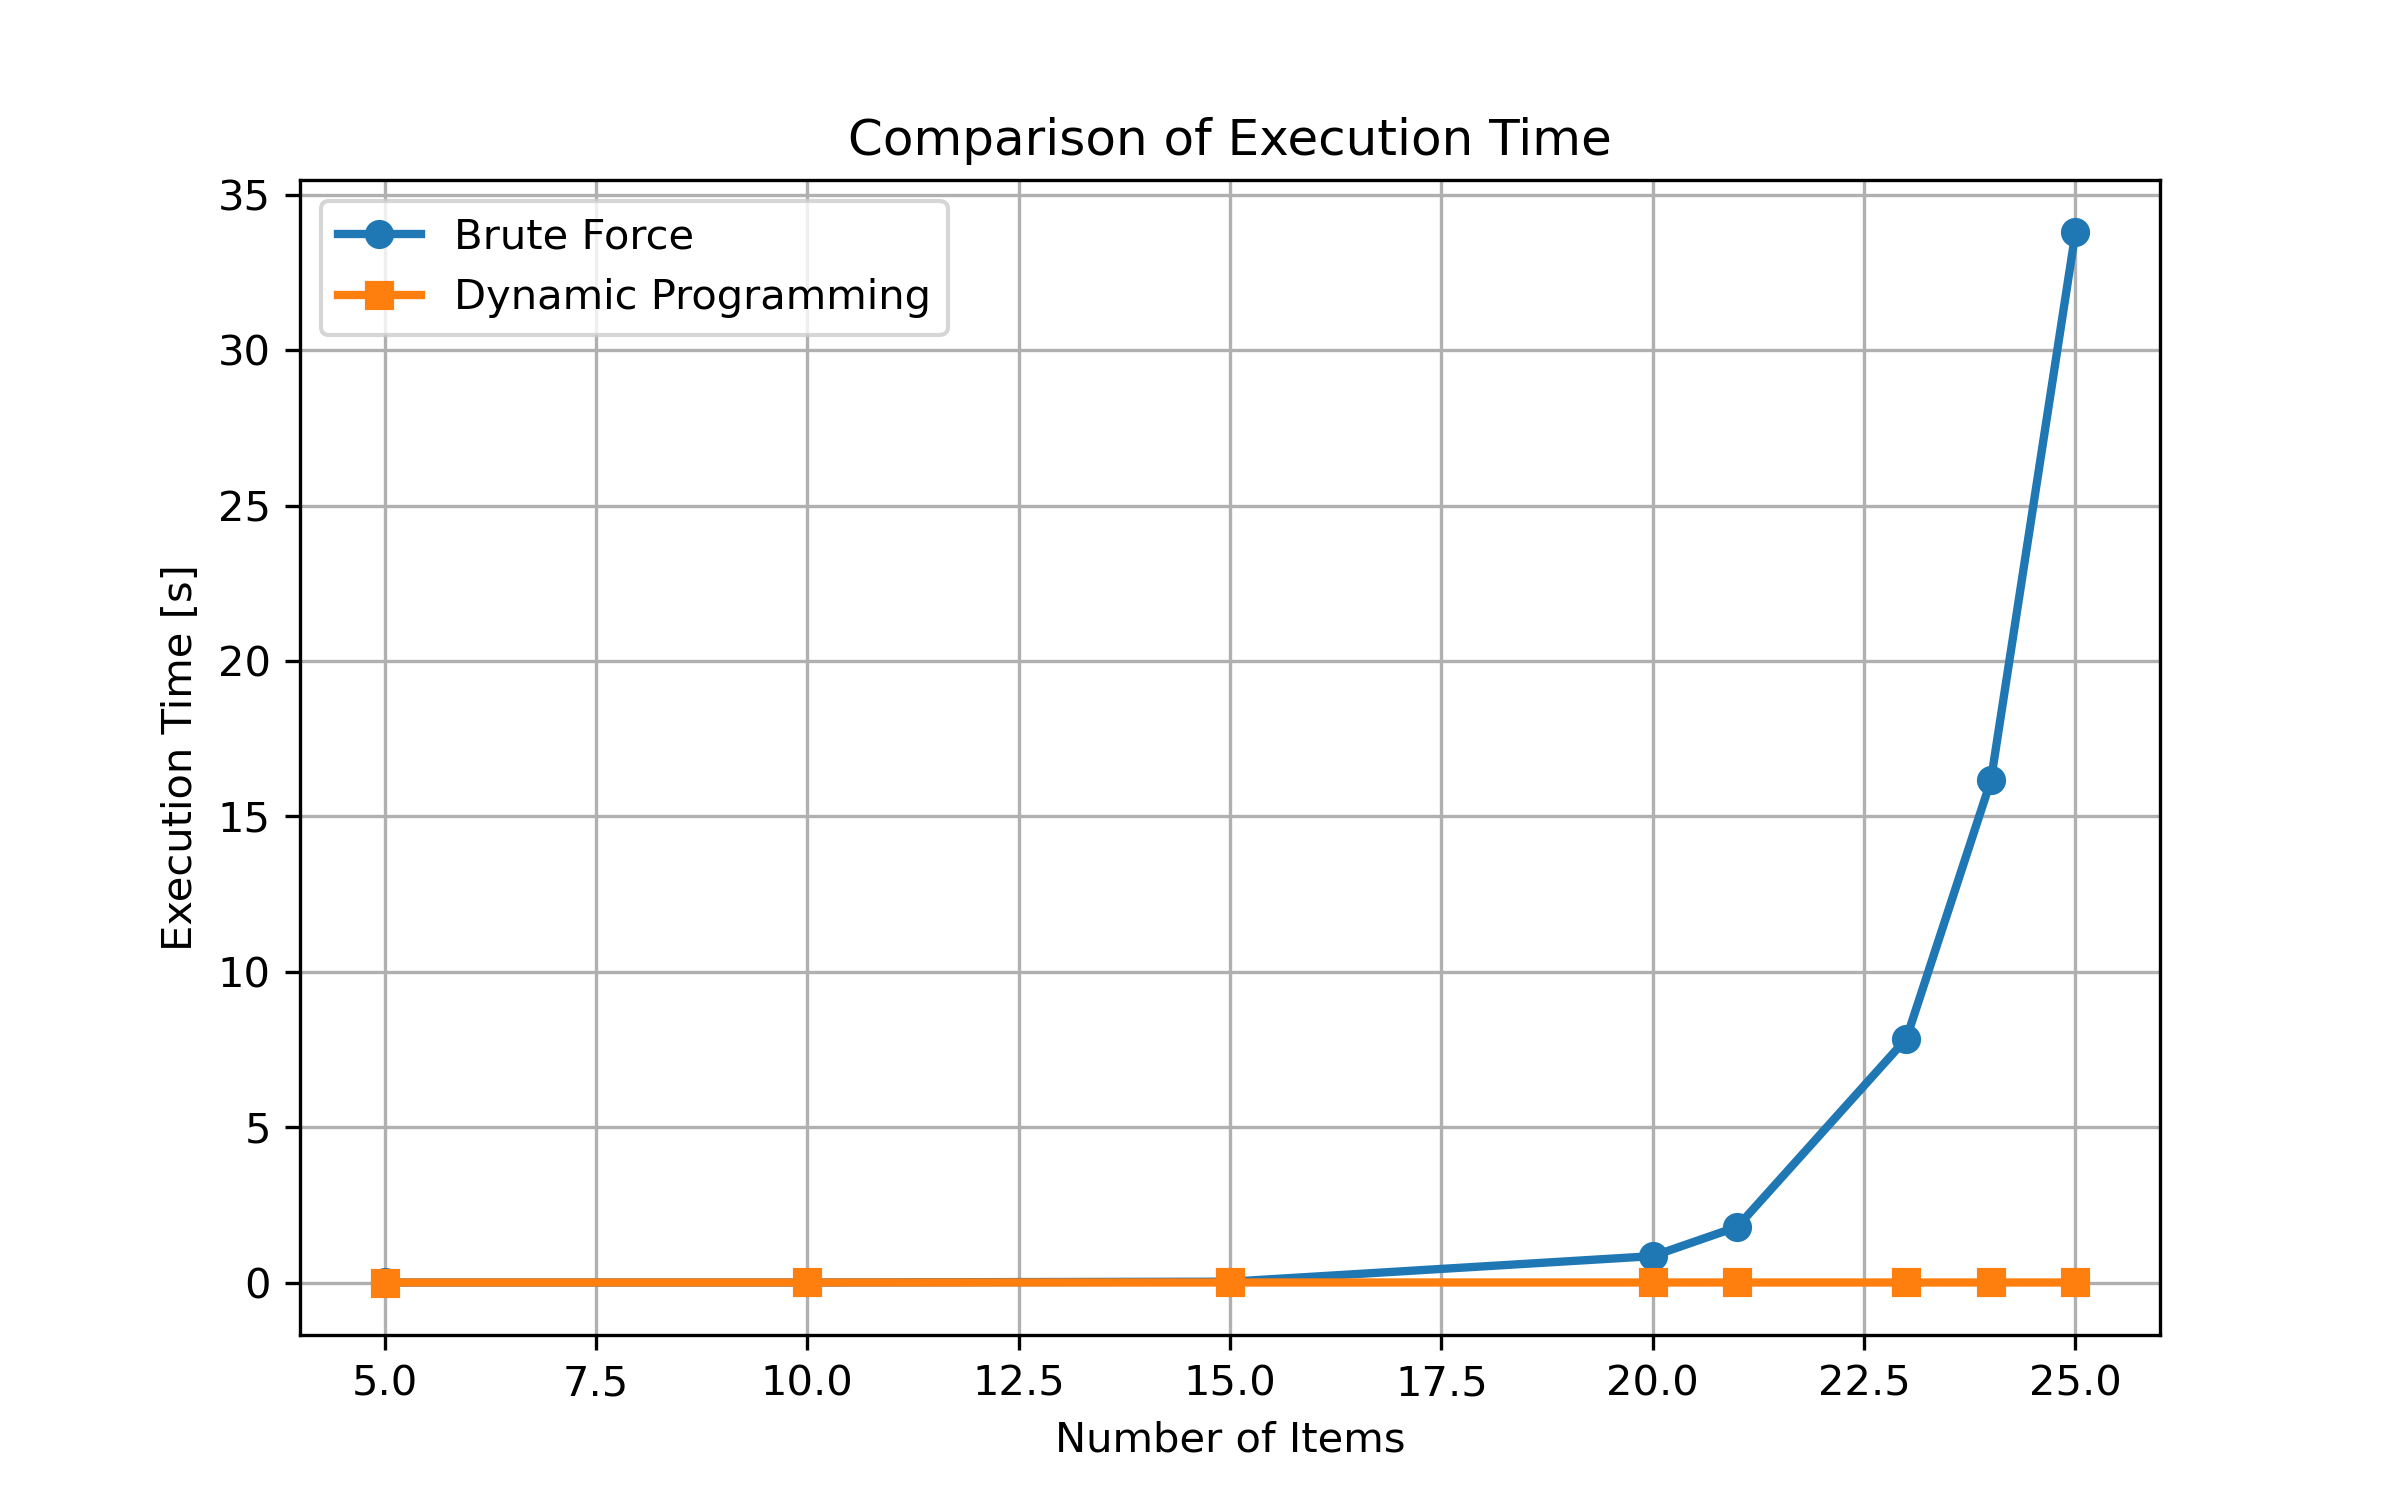
\includegraphics[width=0.85\linewidth]{time_compare.png}
  \caption{総当たり法と動的計画法の実行時間比較}
  \label{fig:time_compare}
\end{figure}

図\ref{fig:time_compare}より、品物数が増えるほど総当たり法は急激に計算量が増えることが分かる。これに対して動的計画法は、重さの上限が大きすぎなければ効率よく解を求めることができる。

\section{考察}

総当たり法は、すべての組み合わせを調べるため、アルゴリズムとしては単純で理解しやすく、必ず最適解を得ることができる。しかし、品物数が増えると組み合わせ数が $2^n$ 通りに増加するため、実行時間が長くなる。

一方、動的計画法では、\texttt{dp[w]} を「重さ $w$ 以内で達成できる最大価値」として保存することで、同じ計算を繰り返さずに済む。そのため、総当たり法よりも効率的に解を求めることができる。

特に、\texttt{dp[w - Weight[i]] + money[i]} という式は、「現在の品物を入れた場合、残りの重さで達成できる最大価値に、現在の品物の価値を加える」という意味である。このように、動的計画法では小さな問題の答えを利用して、大きな問題の答えを求めている。

\section{まとめ}

本レポートでは、ナップサック問題に対して総当たり法と動的計画法を用いて解を求めた。総当たり法はすべての組み合わせを調べるため分かりやすいが、計算量が大きい。一方、動的計画法は途中結果を保存して再利用することで、より効率的に最大価値を求めることができる。

\end{document}